\vspace*{-1.5cm}
\section{Vecteurs du plan}

\subsection{Définition}

\subsubsection{Direction d'une droite, et sens sur une direction de droite}

\begin{itemize}
\item Soit $D$ une droite \\ On appelle \textbf{direction de D} l'ensemble des droites parallèles à $D$.

\item Soit $D$ une droite \\ On dit qu'on a choisi un \textbf{sens sur la direction de $\mathbf{D}$} dès que l'on a orienté toutes les droites  parralèles à $\mathbf{D}$ de la même façon.
\end{itemize}

\subsubsection{Définition fondamentale}

On appelle \textbf{vecteur} la donnée de : \\

\begin{itemize}
\item[*] Une direction de droite ;
\item[*] Un sens sur cette direction ;
\item[*] Un nombre réel positif. \\


\end{itemize}

Plus précisément : Soient A et B deux points distincts.

La donnée \textbf{dans cet ordre} des points A et B définit un vecteur noté $\overrightarrow{AB}$ : \\

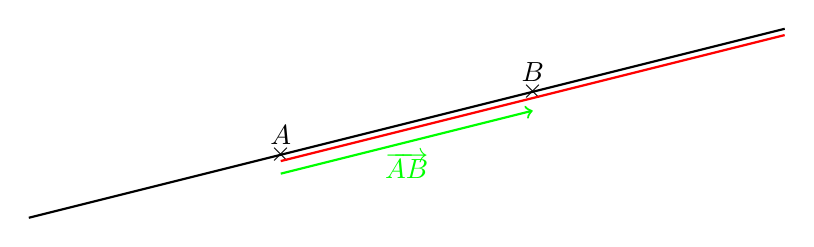
\begin{tikzpicture}[scale=0.8]
\coordinate (A) at (0, 0) ; 
\coordinate (B) at (4, 1) ; 
% Le coef directeur est 1/4 et le vecteur directeur (4 ; 1)     
   
\coordinate (A2) at (0, 0) ; 
\coordinate (B2) at (3, 1) ; 
\coordinate (A3) at (0, 0) ; 
\coordinate (B3) at (3, 1) ; 
\draw[thick] (-4,-1)  -- (8,2) ;
\draw (0,0) node {$\times$} ; \draw (0,0) node [above] {$A$} ;
\draw (4,1) node {$\times$} ; \draw (4,1) node [above] {$B$} ;
    
\draw[thick,red] (0,-0.1)  -- (8,1.9) ;
\draw[thick,green, ->] (0,-0.3)  -- node[midway,below, green]{$ \overrightarrow{AB}$} (4,0.7) ;
\end{tikzpicture}

\begin{itemize}
\item[*] La direction de droite est la direction de la droite $ \left(AB\right) $
\item[*] Le sens sur cete direction est le sens de A vers B, c'est-à-dire le sens de la demi-droite $\left[AB\right)$
\item[*] Le nombre réel positif est la longueur du segment $\left[AB\right]$, c'est-à-dire la distance AB.
\end{itemize}

\subsection{Égalité de 2 vecteurs}

Soient $\overrightarrow{AB}$ et $\overrightarrow{CD}$ deux vecteurs. \\

$\overrightarrow{AB}=\overrightarrow{CD}$ si et seulement si :
\begin{itemize}
\item[*] La direction $(AB) =$ la direction de $(CD)$, c'est-à-dire $(AB)//(CD)$.
\item[*] Le sens de $\left[AB\right) =$ le sens de $\left[CD\right)$
\item[*] La longueur de $[AB] =$ la longueur de $[CD]$
\end{itemize}

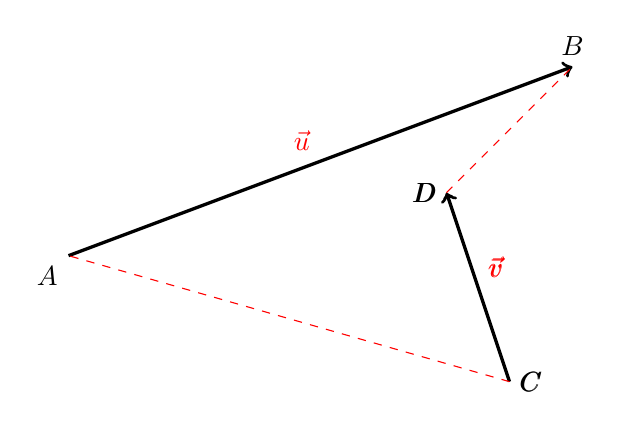
\begin{tikzpicture}[scale=0.8]
\draw[color=black,very thick, ->]
% A(0,0) L'étiquette est à côté de du point.
% Le nom du vecteur u est au dessus à gauche du milieu du trait épais 
(0,2) node [below left] {$A$} --  node[color=red, midway,above left]{$\vec{u}$}
% Le + signifie la translation 
+(8,3) node [above] {$B$} ;
\draw[color=black,very thick,->] (7,0) node [right] {$C$} --  node[color=red, above right]{$\vec{v}$} +(-1,3) node [left] {$D$} ;
\draw[color=black,->] (7,0) node [right] {$C$} --  node[color=red, above right]{$\vec{v}$} +(-1,3) node [left] {$D$} ;
\draw[color=red,dashed] (7,0)  -- (0,2) ;
\draw[color=red,dashed] (6,3)  -- (8,5) ;
\end{tikzpicture}\\
$\overrightarrow{AB} \neq \overrightarrow{CD}$ car $(AB)$ et $(CD)$ ne sont pas parralèles

\newpage



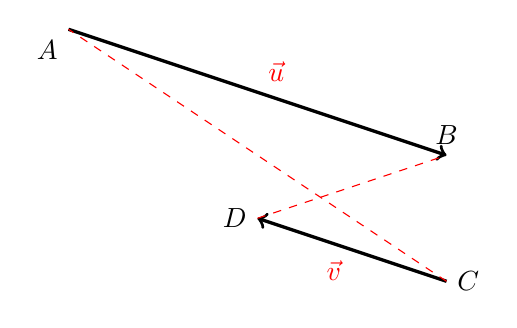
\begin{tikzpicture}[scale=0.8]
\draw[color=black,very thick, ->]
(0,4) node [below left] {$A$} --  node[color=red, midway,above right]{$\vec{u}$}+(6,-2) node [above] {$B$} ;
\draw[color=black,very thick,->] (6,0) node [right] {$C$} --  node[color=red, below left]{$\vec{v}$} +(-3,1) node [left] {$D$} ;
\draw[color=red,dashed] (6,0)  -- (0,4) ;
\draw[color=red,dashed] (3,1)  -- (6,2) ;
\end{tikzpicture}\\


$\overrightarrow{AB} \neq \overrightarrow{CD}$ car $(AB) // (CD)$ mais le sens de $[AB) \neq$ le sens de $[CD)$.

\vspace{1cm}

\begin{tikzpicture}[scale=0.8]
\draw[color=black,very thick, ->]
(5,5) node [below left] {$A$} --  node[color=red, midway,above left]{$\vec{u}$}+(-4,-2) node [above] {$B$} ;
\draw[color=black,very thick,->] (9,5) node [right] {$C$} --  node[color=red, below right]{$\vec{v}$} +(-9,-5) node [left] {$D$} ;
\draw[color=red,dashed] (0,0)  -- (1,3) ;
\draw[color=red,dashed] (5,5)  -- (9,5) ;
\end{tikzpicture}\\

$\overrightarrow{AB} \neq \overrightarrow{CD}$ car $(AB) // (CD)$, le sens de $[AB) = $ le sens de $[CD)$, mais $AB \neq CD$.

\vspace{1cm}

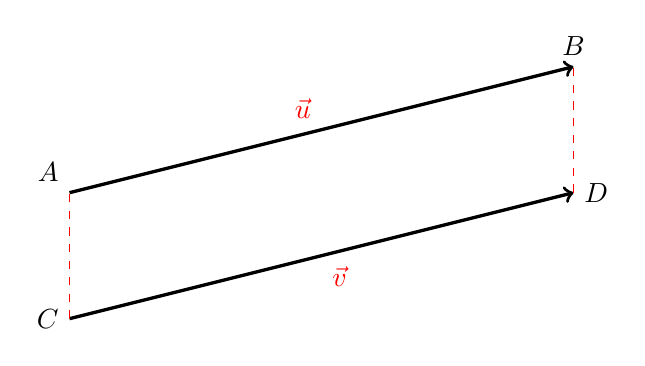
\begin{tikzpicture}[scale=0.8]
\draw[color=black,very thick, ->]
(0,2) node [above left] {$A$} --  node[color=red, midway,above left]{$\vec{u}$}+(8, 2) node [above] {$B$} ;
\draw[color=black,very thick,->] (0,0) node [left] {$C$} --  node[color=red, below right]{$\vec{v}$} +(8, 2) node [right] {$D$} ;
\draw[color=red,dashed] (0,0)  -- (0, 2) ;
\draw[color=red,dashed] (8,2)  -- (8, 4) ;
\end{tikzpicture}\\

$\overrightarrow{AB} = \overrightarrow{CD}$ car $(AB) // (CD)$, le sens de $[AB) = $ le sens de $[CD)$ et $AB = CD$.

$\overrightarrow{u} =\overrightarrow{AB} = \overrightarrow{CD}$

En rouge, le quadrilatère ABDC.

$\overrightarrow{AB} = \overrightarrow{CD} \Longleftrightarrow$ ABDC est un parallélogramme.

Remarques :
\begin{itemize}
\item[*] {\Large $\Longleftrightarrow$} se lit : \og  équivalent à \fg , ou \og  si et seulement si \fg
\item[*] Si $\overrightarrow{AB} = \overrightarrow{CD}$, et ABDC est un parallélogramme, on a aussi :
\begin{itemize}
\item[*]$\overrightarrow{BA} = \overrightarrow{DC}$
\item[*]$\overrightarrow{AC} = \overrightarrow{BD}$
\item[*]$\overrightarrow{CA} = \overrightarrow{DB}$
\end{itemize}
\end{itemize}

\newpage

\subsection{Axiome fondamental}

Soit O un point. 

Soit $\overrightarrow{u}$ un vecteur.

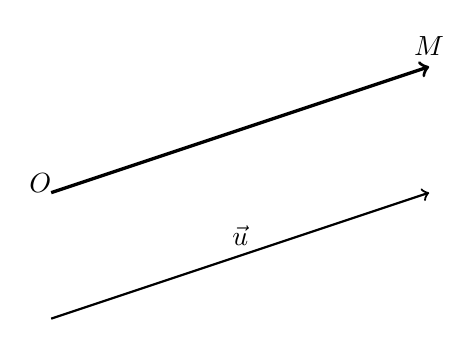
\begin{tikzpicture}[scale=0.8]
\tkzDefPoint [label=left:$O$](0,0){O}
\tkzDrawPoint[size=10,color=black](O)

	\coordinate (M) at (6, 2) ; 

    \draw[very thick,->] (0,0) --  (6,2) node [above] {$M$}  ;
    \draw[thick, ->] (0,-2) -- node[midway,above]{$\vec{u}$} +(6,2);
\end{tikzpicture} \\

Il existe un point M et un seul tel que $\overrightarrow{OM} = \overrightarrow{u}$

\subsection{Addition de vecteurs}

Soit $\vec{u}$ et $\vec{v}$ deux vecteurs.

\begin{tikzpicture}[scale=0.8]
    \coordinate (A) at (0, 0) ; 
    \coordinate (B) at (2, 4) ; 
    \coordinate (C) at (7, 4) ; 	
    \coordinate (C) at (11, 4) ; 	

  \draw[thick,green, ->] (0,0)  --  node[midway,above, green]{$\vec{u}$} +(2,4);
    \draw[thick, ->] (7,4) -- node[midway,above]{$\vec{v}$} +(4,0);

\end{tikzpicture} \\

\subsubsection{Méthode mathématique}

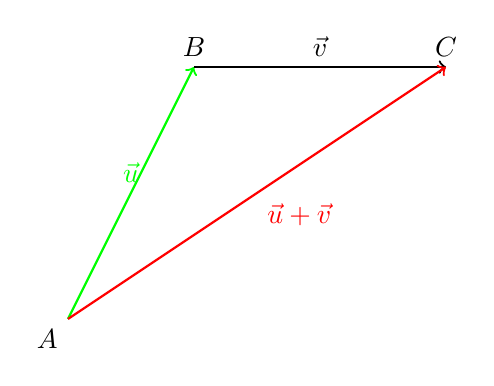
\begin{tikzpicture}[scale=0.8]
    \coordinate (A) at (0, 0) ; 
    \coordinate (B) at (2, 4) ; 
    \coordinate (C) at (2, 4) ; 	
    \coordinate (C) at (6, 4) ; 	
    \draw[thick,green, ->] (0,0) node [below left, black] {$A$} --  node[midway,above, green]{$\vec{u}$} +(2,4) node [above, black] {$B$} ;
    \draw[thick, ->] (2,4) -- node[midway,above]{$\vec{v}$} +(4,0) node [above] {$C$} ;
    \draw[thick,red, ->] (0,0) --  node[midway,below right]{$\vec{u}+\vec{v}$} +(6,4);
\end{tikzpicture}

$\vec{u} + \vec{v} = \overrightarrow{AC}$ \\

$\overrightarrow{AB} + \overrightarrow{BC} = \overrightarrow{AC}$ \\

Ceci s'appelle la \textbf{Relation de Chasles} (Michel Chasles est un mathématicien français (1793-1880)).

\subsubsection{Méthode physique}

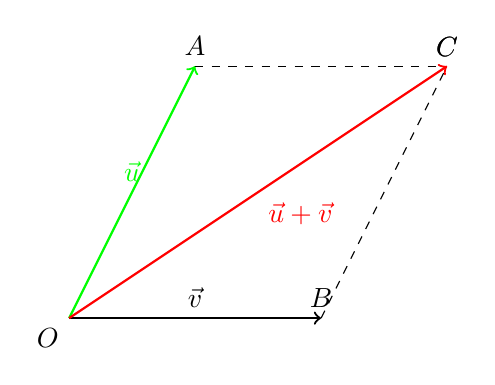
\begin{tikzpicture}[scale=0.8]
    \coordinate (A) at (0, 0) ; 
    \coordinate (B) at (2, 4) ; 
    \coordinate (C) at (2, 4) ; 	
    \coordinate (C) at (6, 4) ; 	
    \draw[thick,green, ->] (0,0) node [below left, black] {$O$} --  node[midway,above, green]{$\vec{u}$} +(2,4) node [above, black] {$A$} ;
    \draw[dashed] (2,4) --  +(4,0) node [above] {$C$} ;
    \draw[thick, ->] (0,0) -- node[midway,above]{$\vec{v}$} +(4,0) node [above] {$B$} ;
    \draw[thick,red, ->] (0,0) --  node[midway,below right]{$\vec{u}+\vec{v}$} +(6,4);
    \draw[dashed] (4,0) --  +(2,4) node [above] {$C$} ;
\end{tikzpicture} 

$\vec{u} + \vec{v} = \overrightarrow{OC}$ \\

$\overrightarrow{OA} + \overrightarrow{OB} = \overrightarrow{OC}$ \\

Ceci est \textbf{la règle du parallélogramme}. Le vecteur
$\overrightarrow{OC}$ s'appelle \textbf{la résultante des forces}. \\

\subsection{Conséquences de la relation de Chasles}

\subsubsection{Le vecteur nul}

Soit A un point. \\

Combien vaut le vecteur $\overrightarrow{AA}$ ? \\


$\overrightarrow{AA} + \overrightarrow{AB} = \overrightarrow{AB}$

$ x + a = a $

$ x = 0 $.

Donc $\overrightarrow{AA} = \overrightarrow{0}$ (<-- vecteur nul) \\

\subsubsection{L'opposé d'un vecteur}

Soient A et B deux points.


Combien vaut le vecteur $\overrightarrow{BA}$ ? \\


$\overrightarrow{AB} + \overrightarrow{BA} = \overrightarrow{AA}$

$\overrightarrow{AB} + \overrightarrow{BA} = \overrightarrow{0}$

$ a + x = 0 $

$ x = - a $

Donc $\overrightarrow{BA} = -\overrightarrow{AB}$ (<-- opposé de $\overrightarrow{AB}$

\subsubsection{Soustraction de deux vecteurs}

\begin{tikzpicture}[scale=0.8]
 \draw[thick,green, ->] (0,0)  --  node[midway,below right , green]{$\vec{u}$} +(2,4);
    \draw[thick, ->] (7,4) -- node[midway,above]{$\vec{v}$} +(4,0);
\end{tikzpicture} 

$\overrightarrow{u} - \overrightarrow{v} = \overrightarrow{u}+\left(-\overrightarrow{v}\right)$

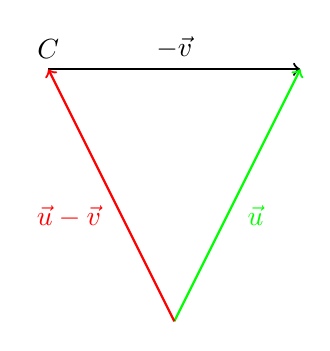
\begin{tikzpicture}[scale=0.8]

    \draw[thick, <-] (0,0) -- node[midway,above]{$-\vec{v}$} +(-4,0) node [above] {$C$} ;
    \draw[thick,green, ->] (-2,-4) --  node[midway,below right, green]{$\vec{u}$} +(2,4);
    \draw[thick,red, ->] (-2,-4) --  node[midway,below left]{$\vec{u}-\vec{v}$} +(-2,4);
\end{tikzpicture} 

\subsection{Multiplication d'un vecteur par un nombre réel}

Soit $\overrightarrow{u}$ un vecteur.

Soit $\lambda$ un nombre réel. 

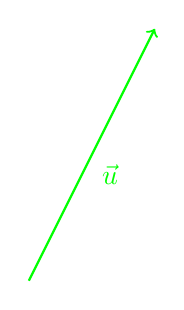
\begin{tikzpicture}[scale=0.8]
 \draw[thick,green, ->] (0,0)  --  node[midway,below right , green]{$\vec{u}$} +(2,4);
\end{tikzpicture} 

Le produit du vecteur $\overrightarrow{u}$ par le nombre réel $\lambda$ est le vecteur noté $\lambda\overrightarrow{u}$ défini par : 

-- La direction de $\left(CD\right) = $ la direction de $\left(AB\right)$, c'est-à-dire $\left(AB\right) // \left(CD\right) $ \\

\begin{tabular}{l|l}

$\lambda > 0 $ & $\lambda < 0$ \\
* Le sens de $\left[CD\right) $ & * le sens de $\left[AB\right) $ \\ 
 $ CD = \lambda AB $ & $ CD = -\lambda AB$ \\
\end{tabular}


\subsubsection{Exemple \no 1}

$\lambda = 3 $

\begin{tikzpicture}[scale=0.6]
\draw[thick,green, ->] (1,2) node [below left] {$A$} --  node[midway,above left, green]{$\vec{u}$} +(1,2) node [above] {$B$} ;
    
\draw[thick,green, ->] (3,0) node [below] {$C$} --  node[midway, below right, green]{$3\vec{u}$} +(3,6) node [above ] {$D$} ;
\draw (4,2) node {$-$} ; \draw (5,4) node {$-$} ; 
\end{tikzpicture}

\subsubsection{Exemple \no 2}

$\lambda = -2 $

\begin{tikzpicture}[scale=0.8]
\draw[thick, ->] (1,2) node [below left] {$A$} --  node[midway,above left]{$\vec{u}$} +(1,2) node [above] {$B$} ;
    
\draw[thick, <-] (3,0) node [below] {$D$} --  node[midway, below right]{$-2\vec{u}$} +(2,4) node [above ] {$C$} ;
\draw (4,2) node {$-$} ; 
\end{tikzpicture}

Et si $\lambda = 0$ ? \\

Alors $0\overrightarrow{u} = \overrightarrow{0}$

\subsection{Notions d'espace vectoriel}

Soient $\overrightarrow{u}$, $\overrightarrow{v}$, et  $\overrightarrow{w}$ trois vecteurs.

Soient $\lambda$ et $\mu$ deux nombres réels. \\

\subsubsection{Relations avec des vecteurs}

\begin{itemize}
\item[*] $\overrightarrow{u} + \overrightarrow{v}$ = $\overrightarrow{v} + \overrightarrow{u}$
\item[*] $\overrightarrow{u} + \left(\overrightarrow{v} + \overrightarrow{w} \right) = \left( \overrightarrow{u} + \overrightarrow{v} \right) + \overrightarrow{w}$
\item[*] $\overrightarrow{u} + \overrightarrow{0} = \overrightarrow{u}$
\item[*] $\overrightarrow{u} + \left(-\overrightarrow{u}\right) = \overrightarrow{0}$
\end{itemize}

\subsubsection{Relations avec des vecteurs et des nombres réels}

\begin{itemize}
\item[*]$1\overrightarrow{u} = \overrightarrow{u}$
\item[*]$\lambda\left(\mu \overrightarrow{u} \right) = \left(\lambda\mu\right)\overrightarrow{u}$
\item[*] $\lambda \times \left( \overrightarrow{u} + \overrightarrow{v}\right) = \lambda \overrightarrow{u} + \lambda \overrightarrow{v}$
\item[*] $\left(\lambda + \mu \right) \overrightarrow{u} = \lambda \overrightarrow{u} + \mu \overrightarrow{u}$
\end{itemize}

\newpage 
\subsection{Vecteurs colinéaires}

\subsubsection{Définition}

Soient $\overrightarrow{u}$ et $\overrightarrow{v}$ deux vecteurs, avec $\overrightarrow{u} \neq \overrightarrow{0}$.

$\overrightarrow{v}$ est colinéaire à $\overrightarrow{u}$ si et seulement si : il existe $\lambda \in \R$ tel que $\overrightarrow{v} = \lambda\overrightarrow{u}$ \\

Exemple :

\begin{tikzpicture}[scale=0.6]
% A(0,0) L'étiquette est à côté de du point.
% Le nom du vecteur u est au dessus à gauche du milieu du trait épais 
\draw[thick, ->] (0,0) node [below left] {$A$} --  node[midway,above left]{$\vec{u}$}
% Le + signifie la translation 
+(2,2) node [above] {$B$} ;

% D(3,0)
\draw[thick, ->] (3,0) node [below] {$D$} --  node[midway, below right]{$\vec{v}$} +(6,6) node [above ] {$C$} ;
% On place deux petites marques pour montrer v = 3u
\draw (5,2) node {$\setminus$} ; 
\draw (7,4) node {$\setminus$} ; 
\end{tikzpicture}

$\overrightarrow{v}$ est coliénaire à $\overrightarrow{u}$ car  $\overrightarrow{v} = 3 \overrightarrow{u}$. \\

\textbf{Remarque}

$\overrightarrow{0}$ est colinéaire à tous les vecteurs du plan. En effet, pour tout vecteur $\overrightarrow{u}$, on a $\overrightarrow{0} = 0 \overrightarrow{u}$ \\

Soient $\overrightarrow{u} \neq \overrightarrow{0}$ et $\overrightarrow{v} \neq \overrightarrow{0}$ tels que $\overrightarrow{v}$ est colinéaire à $\overrightarrow{u}$. Il existe $ \lambda \in \R $ tel que $\overrightarrow{v} = \lambda\overrightarrow{u}$ avec $\lambda \neq 0 $.

On a donc $\overrightarrow{u} = \dfrac{1}{\lambda}\overrightarrow{v}$ et non $\overrightarrow{u} = \dfrac{\overrightarrow{v}}{\lambda}$

\subsubsection{Syntaxe}

On dit que $\overrightarrow{u}$ et $\overrightarrow{v}$ sont colinéaires, ou que $\overrightarrow{v}$ est colinéaire à  $\overrightarrow{u}$. 

\subsubsection{À retenir}

Soient $\overrightarrow{u}$ et $ \overrightarrow{v} $ deux vecteurs 
colinéaires. Il existe un nombre $\lambda \in \R $ tel que $ \overrightarrow{v} = \lambda \overrightarrow{u} $ avec $ \lambda \neq 0$ \\

\begin{tabular}{c|c}

Si $\lambda > 0 $ & Si $\lambda < 0$ \\
$\overrightarrow{u}$ et $\overrightarrow{v}$ sont colinéaires et de même sens & $\overrightarrow{u}$ et $\overrightarrow{v}$ sont colinéaires et de sens contraires.

\end{tabular}

\subsubsection{Points alignés}

Soient A, B et C trois points alignés.\\

A, B et C sont alignés si et seulement si : $ \overrightarrow{AB}$ et $\overrightarrow{AC}$ sont colinéaires.

% Points alignés
\begin{tikzpicture}[scale=0.8]
\draw[thick, ->] (0,0) --  +(5,3)  ;
 \tkzText(0.5,0.3){\textcolor{black}{$\times$}}  % cf ci-dessus
 \tkzText(.5,.7){\textcolor{black}{A}}
 \tkzText(1.5,.9){\textcolor{black}{$\times$}}  % cf ci-dessus
 \tkzText(1.5,1.3){\textcolor{black}{B}}
 \tkzText(4,2.4){\textcolor{black}{$\times$}}  % cf ci-dessus
 \tkzText(3.9,2.8){\textcolor{black}{C}}
\end{tikzpicture}

A, B et C sont alignés car $\overrightarrow{AB}$ et $\overrightarrow{AC}$ sont colinéaires.

\subsubsection{Droites parallèles}

Soient $\left(AB\right)$ et $\left(CD\right)$ deux droites : \\

$\left(AB\right)$ et $\left(CD\right)$ sont parallèles si et seulement si : $\overrightarrow{AB}$ et $\overrightarrow{AC}$ sont colinéaires.

% Droites //
\begin{tikzpicture}[scale=0.8]
% A(0,0) 
\draw[-] (-2,-1) -- +(8,4) ;
\draw[very thick, ->] (0,0) node [below left] {$A$} -- +(4,2) ;
\draw (0,0) node {$\setminus$} ; 
%\draw (2,1) node {$-$} ; 
%\draw (4,2) node {$-$} ; 
%\draw (4,2) node {$\times$} ; 
%\draw (4,2) node {$\times$} ; 
\draw (4,2) node [above]{$B$} ; 
% D(3,0)
\draw[-] (2,-1) -- +(8,4) ;
\draw[very thick, ->] (4,0) node [below] {$C$} --   +(1, .5) node [above ] {$D$} ;
\end{tikzpicture}

$\left(AB\right) // \left(CD\right) $ car $\overrightarrow{CD} = \dfrac{1}{4} \overrightarrow{AB}$

\subsection{Milieu d'un segment}

\subsubsection{Définition}

Soient A et B deux points distincts.

Il existe un point I et un seul tel que $\overrightarrow{IA} + \overrightarrow{IB} = \overrightarrow{0}$, c'est-à-dire $\overrightarrow{AI} = \dfrac{1}{2} \overrightarrow{AB} $

I est le milieu de $\left[AB\right]$

% milieu d'un segmeny
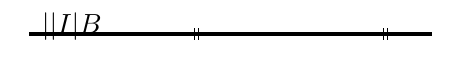
\begin{tikzpicture}[scale=0.8]
\draw[very thick, -] (-.2,0) --  +(6.4,0)  ;
 \tkzText(0,0){\textcolor{black}{$|$}}  % cf ci-dessus
 \tkzText(0,.5){\textcolor{black}{A}}
 \tkzText(3,0){\textcolor{black}{$|$}}  % cf ci-dessus
 \tkzText(3,.5){\textcolor{black}{$I$}}
 \tkzText(6,0){\textcolor{black}{$|$}}  % cf ci-dessus
 \tkzText(6,.5){\textcolor{black}{$B$}}
\draw (1.47,0.09) -- (1.47,-0.09);
\draw (1.54,0.09) -- (1.54,-0.09);
\draw (4.47,0.09) -- (4.47,-0.09);
\draw (4.54,0.09) -- (4.54,-0.09);
\end{tikzpicture}

\subsubsection{Démonstration}

$\overrightarrow{IA} + \overrightarrow{IB} = \overrightarrow{0} $\\

$ \overrightarrow{IA} + \left(\overrightarrow{IA} + \overrightarrow{AB}\right) = \overrightarrow{0} $\\

$ 2\overrightarrow{IA} + \overrightarrow{AB} = \overrightarrow{0} $\\

$ 2\overrightarrow{IA} = -\overrightarrow{AB} $\\

$\overrightarrow{IA} = -\dfrac{1}{2} \overrightarrow{AB} $\\

$ \overrightarrow{AI} = \dfrac{1}{2} \overrightarrow{AB} $\\

\newpage 

\subsection{Centre de gravité d'un triangle}

Soient A, B et C trois points non-alignés.

Il existe un point G et un seul tel que $\overrightarrow{GA} + \overrightarrow{GB} + \overrightarrow{GC} = \overrightarrow{0} $, c'est-à-dire $\overrightarrow{AG} = \dfrac{1}{3} \overrightarrow{AB} + \dfrac{1}{3} \overrightarrow{AC} $ \\

\subsubsection{Démonstration}

$\overrightarrow{GA}+\overrightarrow{BG}+\overrightarrow{GC}=\overrightarrow{0}$\\

$ \overrightarrow{GA} + \left(\overrightarrow{GA} + \overrightarrow{AB} \right) + \left(\overrightarrow{GA} + \overrightarrow{AC}\right) = \overrightarrow{0} $\\

$ 3\overrightarrow{GA} = -\overrightarrow{AB} - \overrightarrow{AC} $\\

$ \overrightarrow{GA} = -\dfrac{1}{3} \overrightarrow{AB} - \dfrac{1}{3} \overrightarrow{AC} $\\

$ \overrightarrow{AG} = \dfrac{1}{3} \overrightarrow{AB} + \dfrac{1}{3} \overrightarrow{AC} $\\

\subsubsection{Propriété fondamentale}

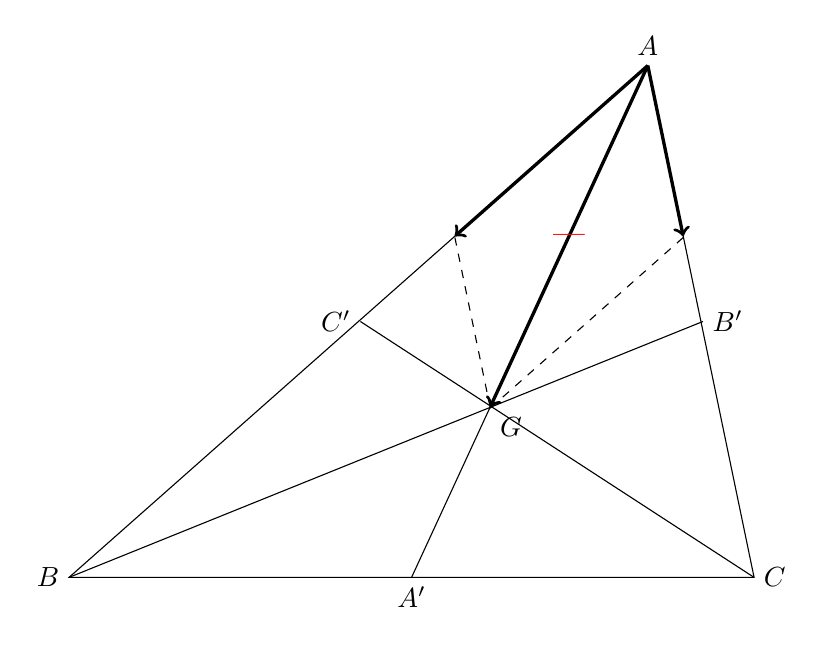
\begin{tikzpicture}[scale=0.5]
\coordinate (G) at (0.2,-0.07) ; 

\draw (6,8) node [above] {$A$} --  (-8.7,-5) node [left] {$B$} -- (8.7,-5) node [right] {$C$}-- (6, 8) ; 
\draw (6,8) -- (0,-5) node [below] {$A'$} ;
\draw (-8.7,-5) -- (7.4,1.5) node [right] {$B'$} ;
\draw (8.7,-5) -- (-1.3,1.5) node [left] {$C'$} ;
\draw (2,-0.7) node [below right] {$G$} ; 

\draw [very thick, ->](6,8) -- +(-14.7/3, -13/3) ; % 1/3 de vec(AB)
\draw [dashed](2, -0.7) -- +(-2.7/3, 13/3) ;       % 1/3 de vec(-AC)
\draw [very thick, ->](6,8) -- +(2.7/3, -13/3) ;   % 1/3 de vec(AC)
\draw [dashed](2, -0.7) -- +(14.7/3, 13/3) ;       % 1/3 de vec(-AB)
\draw [very thick, ->](6,8) -- +(-12/3, -26/3) ;   % 2/3 de vec(AA')
\draw [very thick, red] (4,7.3/2) node {\bf ---} ; % 1/2 de AG 

\end{tikzpicture}

Soit A' le milieu de $\left[BC\right]$

$ \overrightarrow{AG} = \dfrac{1}{3} \overrightarrow{AB} + \dfrac{1}{3} \overrightarrow{AC} $\\

$ \overrightarrow{AG} = \dfrac{1}{3} \left(\overrightarrow{AA'} + \overrightarrow{A'B}\right) + \dfrac{1}{3} \left(\overrightarrow{AA'} + \overrightarrow{A'C} \right) $ \\

$ \overrightarrow{AG} = \dfrac{2}{3} \overrightarrow{AA'} + \dfrac{1}{3} \underbrace{\left(\overrightarrow{A'B} + \overrightarrow{A'C}\right)}_{= \overrightarrow{0} \textrm {car} A' \textrm {est le milieu de} \left[BC\right]} $\\

$ \overrightarrow{AG} = \dfrac{2}{3} \overrightarrow{AA'} $\\

On aussi, avec B' le milieu de $\left[AC\right]$, on a $\overrightarrow{BG} = \dfrac{2}{3} \overrightarrow{BB'} $, et avec C' le milieu de $\left[AB\right]$, on a $\overrightarrow{CG} = \dfrac{2}{3} \overrightarrow{CC'} $

Les trois médianes du triangle sont concourantes en un point, ici G.

\newpage

\subsection{Exercices}

\subsubsection{Exercice \no 0}

Soit ABC un triangle. \\

1. Soit A' le milieu de $\left[BC\right]$. Montrer que $\overrightarrow{AB} + \overrightarrow{AC} = 2\overrightarrow{AA'}$. \\

2. Soient I le milieu de $\left[AB\right]$ et J le milieu de $\left[AC\right]$. Montrer que $\overrightarrow{IJ} = \dfrac{1}{2} \overrightarrow{BC}$.

\begin{tikzpicture}[scale=0.3]
\draw (6,8) node [above] {$A$} --  (-8.7,-5) node [left] {$B$} -- (8.7,-5) node [right] {$C$} -- (6, 8) ; 
\draw [red,->](6,8) -- +(-12, -26) node [midway,below right] {$A'$} node [below] {$G$} ;

\draw [green, ->] (-1.3, 1.5) node [left] {$I$} -- (7.4,1.5) node [right] {$J$} ;

\draw [dashed] (-8.7, -5) -- +(2.7,-13) ;     % ie vec(AC)
\draw [dashed] (8.7, -5) -- +(-14.7,-13) ;     % ie vec(AB)

\end{tikzpicture}

1. $\overrightarrow{AB} + \overrightarrow{AC} = \left(\overrightarrow{AA'} + \overrightarrow{A'B}\right) + \left(\overrightarrow{AA'} + \overrightarrow{A'C}\right) $\\

$ \overrightarrow{AB} + \overrightarrow{AC} = 2 \overrightarrow{AA'} + \underbrace{\overrightarrow{A'B} + \overrightarrow{A'C}}_{= \overrightarrow{0} \textrm{ car } A' \textrm { est le milieu de } \left[BC\right]} $

$ \overrightarrow{AB} + \overrightarrow{AC} = 2 \overrightarrow{AA'} $\\

Donc les diagonales du parallélogramme se coupent en leur milieu. \\

2. $ \overrightarrow{IJ} = \overrightarrow{IA} + \overrightarrow{AJ} $\\

$ \overrightarrow{IJ} = -\overrightarrow{AI} + \overrightarrow{AJ} $\\

$ \overrightarrow{IJ} = -\dfrac{1}{2} \overrightarrow{AB} + \dfrac{1}{2} \overrightarrow{AC} $\\

$ \overrightarrow{IJ} = \dfrac{1}{2} \left(-\overrightarrow{AB} + \overrightarrow{AC} \right) $\\

$ \overrightarrow{IJ} = \dfrac{1}{2} \left(\overrightarrow{BA} + \overrightarrow{AC}\right) $\\

$ \overrightarrow{IJ} = \dfrac{1}{2} \overrightarrow{BC} $
\newpage
\subsubsection{Un superbe exercice}

Soit ABC un triangle.

Soit A' le milieu de $\left[BC\right]$.

Soit G le centre de gravité de ABC.

Soit M un point quelconque.\\

1. Montrer que $ \overrightarrow{MA} + \overrightarrow{MB} + \overrightarrow{MC} = 3\overrightarrow{MA} + 2\overrightarrow{AA'}$

2. Montrer que $ \overrightarrow{MA} + \overrightarrow{MB} + \overrightarrow{MC} = 3\overrightarrow{MG} $

\begin{tikzpicture}[scale=0.7]
\draw (0,8) node [left] {$A$} --  (8,4) node [below] {$B$} -- (12,16) node [right] {$C$} -- (0, 8) ; 
\draw [thick, ->] (0,8) -- +(10,2) node [right] {$A'$} ;   
\draw [dashed] (8,4) -- +(-2,8) ;   
\draw [dashed] (12,16) -- +(-8,-10);   
\draw (20/3, 18/2) node [below] {$G$} ; 

\draw [blue, ->] (0,12) node [left] {$M$} -- +(0,-4) ; 
\draw [green, ->] (0,12) node [left] {$M$} -- +(8,-8) ; 
\draw [violet, ->] (0,12) node [left] {$M$} -- +(12,4) ; 

\draw [thick, blue, ->] (0,12) node [left] {$M$} -- +(0,-12) ; 
\draw [black, ->] (0,0) --  +(20,4) ; 
\draw [red, ->] (0,12) -- +(20, -8) ; 

\draw [green, ->] (0,8) -- +(8,-8) ; 
\draw [violet, ->] (8,0) -- +(12,4) ; 

\end{tikzpicture}

\vspace*{1cm}

\begin{enumerate}


\item $\overrightarrow{MA} + \overrightarrow{MB} + \overrightarrow{MC} = \overrightarrow{MA} + \left(\overrightarrow{MA} + \overrightarrow{AA'} + \overrightarrow{A'B}\right) + \left(\overrightarrow{MA} + \overrightarrow{AA'} + \overrightarrow{A'C}\right) $\\

$ \overrightarrow{MA} + \overrightarrow{MB} + \overrightarrow{MC} = 3\overrightarrow{MA} + 2\overrightarrow{AA'} +$\hspace*{-0.94cm}$ \underbrace{\overrightarrow{A'B} + \overrightarrow{A'C}}_{= \overrightarrow{0} \textrm{ car } A' \textrm{ est le milieu de } \left[BC\right]}$ 

\item  $ \overrightarrow{MA} + \overrightarrow{MB} + \overrightarrow{MC} = \left(\overrightarrow{MG} + \overrightarrow{GA}\right) + \left(\overrightarrow{MG} + \overrightarrow{GB} \right) + \left(\overrightarrow{MG} + \overrightarrow{GC} \right) $\\

$ \overrightarrow{MA} + \overrightarrow{MB} + \overrightarrow{MC} =
3\overrightarrow{MG} + $\hspace*{-1.8cm}$\underbrace{\overrightarrow{GA} + \overrightarrow{GB} + \overrightarrow{GC}}_{=\overrightarrow{0} \textrm{car } G \textrm { est le centre de gravité du triangle } ABC} $

\end{enumerate}
\newpage
\subsubsection{Exercice \no 1}

Soit ABC un triangle.

1. Construire les points M et N définis par : \\

\begin{itemize}
\item[*] $ \overrightarrow{AM} = \dfrac{1}{3} \overrightarrow{AB} + \overrightarrow{AC} $ \\
\item[*] $ \overrightarrow{AN} = 2\overrightarrow{AB} - \dfrac{2}{3} \overrightarrow{AC} $ \\
\end{itemize}

2. Exprimer $\overrightarrow{MN}$ en fonction de $\overrightarrow{AB}$ et de $\overrightarrow{AC}$. \\

3. Montrer que les droites $\left(MN\right)$ et $\left(BC\right)$ sont parallèles. \\

\begin{enumerate}


\item ~   % Le tilde (~) est nécessaire pour que le numéro précède la figure

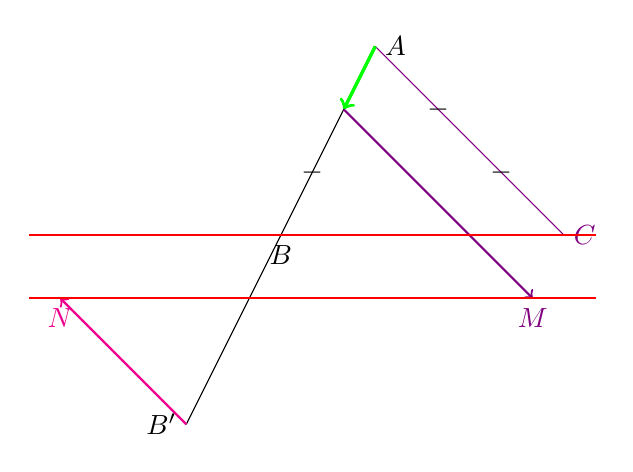
\begin{tikzpicture}[scale=0.2]
\draw [color=black] (0,0) node [left] {$B'$} --  (6,12) node [below] {$B$} -- (12,24) node [right] {$A$} ; 
\draw [color=violet] (12,24) -- +(+12, -12)  node [right] {$C$} ; 
\draw [color=black] (24,12) -- (6, 12) ; 
\draw (8,16) node {$-$} ;   
\draw (16,20) node {$-$} ;   
\draw (20,16) node {$-$} ;   

\draw [color=green, very thick, ->] (12, 24) -- +(-2,-4) ; 
\draw [color=violet, thick, ->] (10, 20) -- +(12,-12) node [below] {$M$} ; 
\draw [color=magenta, thick, ->] (0, 0) -- +(-8,8) node [below] {$N$} ; 

\draw [color=red, thick, -] (-10, 12) -- (26,12) ; 
\draw [color=red, thick, -] (-10, 8) -- (26,8) ; 

\end{tikzpicture}\\


\item  $\overrightarrow{MN} = \overrightarrow{MA} + \overrightarrow{AN} $\\

$ \overrightarrow{MN} = -\overrightarrow{AM} + \overrightarrow{AN} $\\

$ \overrightarrow{MN} = -\dfrac{1}{3} \overrightarrow{AB} - \overrightarrow{AC} + 2\overrightarrow{AB} - \dfrac{2}{3} \overrightarrow{AC} $\\

$ \overrightarrow{MN} = \dfrac{5}{3} \overrightarrow{AB} - \dfrac{5}{3} \overrightarrow{AC} $\\

$ \overrightarrow{MN} = \dfrac{5}{3} \left(\overrightarrow{AB} - \overrightarrow{AC}\right) $\\

\item  $ \overrightarrow{MN} = \dfrac{5}{3} \left(\overrightarrow{AB} - \overrightarrow{AC} \right)$\\

$ \overrightarrow{MN} = \dfrac{5}{3} \left(\overrightarrow{AB} + \overrightarrow{CA} \right)$\\

$ \overrightarrow{MN} = \dfrac{5}{3} \left(\overrightarrow{CA} + \overrightarrow{AB} \right)$\\

$ \overrightarrow{MN} = \dfrac{5}{3} \left(\overrightarrow{CB} \right)$\\

$ \overrightarrow{MN} = -\dfrac{5}{3} \left(\overrightarrow{BC}\right)$\\

Les vecteurs $\overrightarrow{MN}$ et $\overrightarrow{BC}$ sont colinéaires, donc $\left(MN\right)//\left(BC\right)$
\end{enumerate}
\newpage
\subsubsection{Exercice \no 2}

Soit ABC un triangle.

\begin{enumerate}


\item  Construire les points I, J et K définis par :

\begin{itemize}
\item[*] $\overrightarrow{AI} = \dfrac{1}{3} \overrightarrow{AB}$\\
\item[*] $\overrightarrow{BJ} = \dfrac{1}{2} \overrightarrow{BA} - \dfrac{1}{4} \overrightarrow{BC}$\\
\item[*] $\overrightarrow{CK} = -\overrightarrow{AB} - \dfrac{1}{2} \overrightarrow{BC}$\\
\end{itemize}

\item  Exprimer $\overrightarrow{IJ}$ fonction de $\overrightarrow{AB}$ et de $ \overrightarrow{BC}$. 

Puis, exprimer $\overrightarrow{IK}$ en fonction de $\overrightarrow{AB}$ et de $\overrightarrow{BC}$.

\item  Montrer que les points I, J et K sont alignés.

\end{enumerate}

~

\begin{enumerate}

\item  ~ % (Garder là le tilde) Exercice n°2 

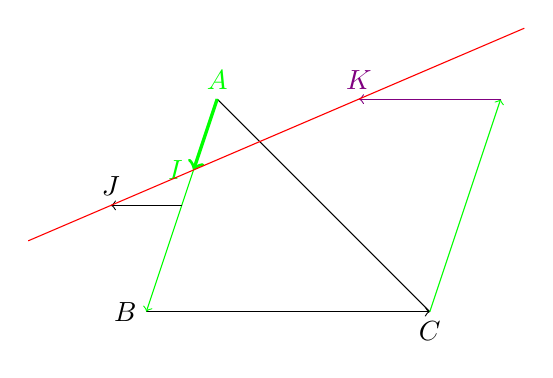
\begin{tikzpicture}[scale=0.3]

\draw [->] (0, 0) node [left] {$B$} --  +(12, 0) node [below] {$C$} ; 
\draw [color=green, <-] (0, 0) -- +(3, 9) node [above] {$A$} ; 
\draw      (3, 9) --  (12, 0); 

\draw [very thick, color=green, ->] (3, 9) -- +(-1, -3) node [left] {$I$} ; 
\draw [->] (3/2, 9/2) -- +(-3, 0) node [above] {$J$} ; 
\draw [color=green, ->] (12, 0) -- +(3, 9); 
\draw [color=violet, ->] (15, 9) -- +(-6, 0) node [above] {$K$} ; 
\draw [color=red] (2, 6) -- +(14, 6) -- +(-7, -3); 

\end{tikzpicture}\\

\begin{multicols}{2}


\item  {\small $\overrightarrow{IJ} = \overrightarrow{IA} + \overrightarrow{AB} + \overrightarrow{BJ} $\\

$\overrightarrow{IJ} = -\dfrac{1}{3} \overrightarrow{AB} + \overrightarrow{AB} + \dfrac{1}{2} \overrightarrow{BA} - \dfrac{1}{4} \overrightarrow{BC} $\\

$\overrightarrow{IJ} = -\dfrac{1}{3} \overrightarrow{AB} + \overrightarrow{AB} - \dfrac{1}{2} \overrightarrow{AB} - \dfrac{1}{4} \overrightarrow{BC} $\\

$ \overrightarrow{IJ} = \dfrac{1}{6} \overrightarrow{AB} - \dfrac{1}{4} \overrightarrow{BC} $\\

Et : $\overrightarrow{IK} = \overrightarrow{IA} + \overrightarrow{AB} + \overrightarrow{BC} + \overrightarrow{CK} $\\

$ \overrightarrow{IK} = -\dfrac{1}{3} \overrightarrow{AB} + \overrightarrow{AB} + \overrightarrow{BC} - \overrightarrow{AB} - \dfrac{1}{2} \overrightarrow{BC} $\\

$ \overrightarrow{IK} = -\dfrac{1}{3} \overrightarrow{AB} + \dfrac{1}{2} \overrightarrow{BC} $\\

\item $\overrightarrow{IK} = \overrightarrow{IB} + \overrightarrow{BC} + \overrightarrow{BA} + \dfrac{1}{2} \overrightarrow{CB} $\\

$ \overrightarrow{IK} = \dfrac{2}{3} \overrightarrow{AB} + \overrightarrow{BC} - \overrightarrow{AB} - \dfrac{1}{2} \overrightarrow{BC} $\\

$ \overrightarrow{IK} = -\dfrac{1}{3} \overrightarrow{AB} + \dfrac{1}{2} \overrightarrow{BC} $\\

On constate que $\overrightarrow{IK} = -2\left(\dfrac{1}{6} \overrightarrow{AB} + \dfrac{1}{2} \overrightarrow{BC}\right) $\\

$ \overrightarrow{IK} = -2\overrightarrow{IJ} $
}\\

Donc les vecteurs $\overrightarrow{IK}$ et $\overrightarrow{IJ}$ sont colinéaires, donc les points I, J et K sont alignés.

\end{multicols} 
\end{enumerate}
\newpage
\subsubsection{Exercice \no 3}

Soit ABC un triangle.

\begin{enumerate}


\item  Construire les points I et J tels que :

\begin{itemize}
\item[*] $\overrightarrow{AI} = -2\overrightarrow{AB}$\\
\item[*] $\overrightarrow{AJ} = - \overrightarrow{AB} + \dfrac{1}{2} \overrightarrow{AC}$\\
\end{itemize}

\item  Montrer que J et le milieu de $\left[IC\right]$
\end{enumerate}



\begin{enumerate}

 \item ~ \\% Exercice n°3 (suite) 
 
\begin{tikzpicture}[scale=.4]

\draw [color=black] (0, 0) node [left] {$B$} --  (6, 6) node [left] {$A$} ; 
\draw [color=green, ->] (6, 6) -- +(4, -6) node [right] {$C$} ; 
\draw (0, 0) --  (10, 0); 
\draw [color=green, ->] (6, 6) -- +(2, -3); 
\draw [color=violet, ->] (6, 6) -- +(12, 12) node [right] {$I$} ; 
\draw [color=red, ->] (10, 0) -- +(8, 18); 
\draw [color=green, ->] (12, 12) -- +(2, -3) node [right] {$J$} ; 
\end{tikzpicture}

\vspace*{1cm}


\item $\overrightarrow{JI} + \overrightarrow{JC} = \left(\overrightarrow{JA} + \overrightarrow{AI}\right) + \left(\overrightarrow{JA} + \overrightarrow{AC}\right) $

$ \overrightarrow{JI} + \overrightarrow{JC} = \overrightarrow{AB} - \dfrac{1}{2} \overrightarrow{AC} + \overrightarrow{AI} +\overrightarrow{AB} - \dfrac{1}{2} \overrightarrow{AC} + \overrightarrow{AC} $

$\overrightarrow{JI} + \overrightarrow{JC} = 2\overrightarrow{AB} + \overrightarrow{AI} $

$ \overrightarrow{JI} + \overrightarrow{JC} = 2\overrightarrow{AB} + \left(-2\right)\overrightarrow{AB} $

$ \overrightarrow{JI} + \overrightarrow{JC} = \overrightarrow{0} $

Donc J est le milieu de $\left[IC\right]$.

\end{enumerate}

\newpage
\subsubsection{Exercice \no 4}

Soit ABC un triangle.

Soient A' le milieu de $\left[BC\right]$, B' le milieu de $\left[AC\right]$, et C' le milieu de $\left[AB\right]$

Soit G le centre de gravité de ABC.

\begin{enumerate}


\item  Exprimer :

\begin{itemize}
\item[*] $\overrightarrow{AB} + \overrightarrow{AC} $ en fonction de $\overrightarrow{AA'}$\\
\item[*] $\overrightarrow{BA} + \overrightarrow{BC}$ en fonction de $\overrightarrow{BB'}$\\
\item[*] $\overrightarrow{CA} + \overrightarrow{CB}$ en fontion de $\overrightarrow{CC'}$\\
\end{itemize}

\item Montrer que $\overrightarrow{AA'} + \overrightarrow{BB'} + \overrightarrow{CC'} = \overrightarrow{0} $

\item  Montrer que $G$ est le centre de gravité du triangle A'B'C'.
\end{enumerate}



\begin{enumerate}

\item ~ 

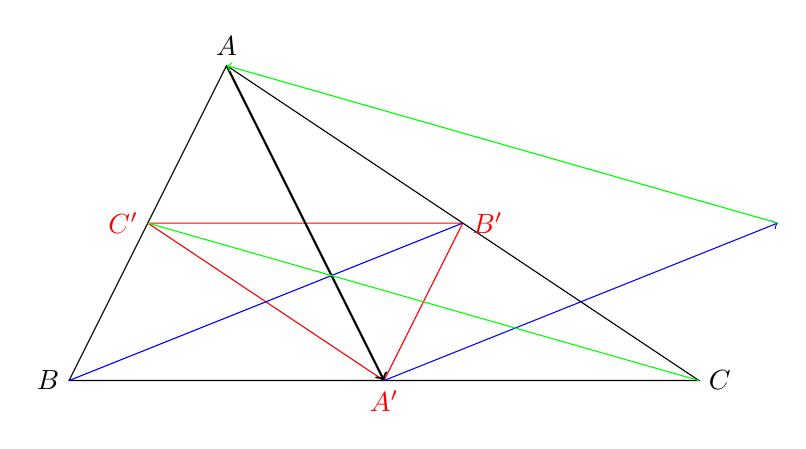
\begin{tikzpicture}[scale=1]
\draw (0,0) node [left] {$B$} -- (2,4) node [above] {$A$} -- (8,0) node [right] {$C$} -- cycle ;  
\draw [red] (1,2) node [left] {$C'$} -- (5,2) node [right] {$B'$} -- (4,0) node [below] {$A'$} -- cycle ; 
\draw [thick, ->] (2,4) -- (4,0) ; 
\draw [blue, ->] (0,0) -- +(5,2) (4,0) -- +(5,2) ; 
\draw [green, ->] (8,0) -- +(-7,2) (9,2) -- +(-7,2) ; 
\end{tikzpicture}


 $\overrightarrow{AB} + \overrightarrow{AC} = \left(\overrightarrow{AA'} + \overrightarrow{A'B}\right) + \left(\overrightarrow{AA'} + \overrightarrow{A'C}\right) $\\

$ \overrightarrow{AB} + \overrightarrow{AC} = 2\overrightarrow{AA'} + \underbrace{\overrightarrow{A'B} + \overrightarrow{A'C}}_{= \overrightarrow{0} \textrm { car } A' \textrm { est le milieu de } \left[BC\right]}$\\

$\overrightarrow{AB} + \overrightarrow{AC} = 2\overrightarrow{AA'} $\\

Donc $\overrightarrow{BA} + \overrightarrow{BC} = 2\overrightarrow{BB'} $ et $ \overrightarrow{CA} + \overrightarrow{CB} = 2\overrightarrow{CC'} $\\

\item  $\overrightarrow{AA'} + \overrightarrow{BB'} + \overrightarrow{CC'} = \dfrac{1}{2} \left(\overrightarrow{AB} + \overrightarrow{AC} \right) + \dfrac{1}{2} \left(\overrightarrow{BA} + \overrightarrow{BC} \right) + \dfrac{1}{2} \left( \overrightarrow{CA} + \overrightarrow{CB} \right) $\\

$\overrightarrow{AA'} + \overrightarrow{BB'} + \overrightarrow{CC'} = \dfrac{1}{2} \overrightarrow{AB} + \dfrac{1}{2} \overrightarrow{BA} + \dfrac{1}{2} \overrightarrow{AC} + \dfrac{1}{2} \overrightarrow{CA} + \dfrac{1}{2} \overrightarrow{BC} + \dfrac{1}{2} \overrightarrow{CB} $\\

$ \overrightarrow{AA'} + \overrightarrow{BB'} + \overrightarrow{CC'} = \dfrac{1}{2} \overrightarrow{AA} + \dfrac{1}{2} \overrightarrow{AA} + \dfrac{1}{2} \overrightarrow{BB} $

$ \overrightarrow{AA'} + \overrightarrow{BB'} + \overrightarrow{CC'} = \overrightarrow{0} $\\

\item $\overrightarrow{GA'} + \overrightarrow{GB'} + \overrightarrow{GC'} = \left(\overrightarrow{GA} + \overrightarrow{AA'} \right) + \left(\overrightarrow{GB} + \overrightarrow{BB'} \right) + \left(\overrightarrow{GC} + \overrightarrow{CC'} \right) $\\

$ \overrightarrow{GA'} + \overrightarrow{GB'} + \overrightarrow{GC'} = \underbrace{\overrightarrow{GA} + \overrightarrow{GB} + \overrightarrow{GC}}_{=\overrightarrow{0} \textrm { car } G \textrm { est le centre de gravité de }  ABC} + \underbrace{\overrightarrow{AA'} + \overrightarrow{BB'} + \overrightarrow{CC'}}_{=\overrightarrow{0} \textrm { d'après } 2.} $\\

Donc G est le centre de gravité du triangle A'B'C'.
\end{enumerate}
\newpage
\subsubsection{Exercice \no 5}

Soit ABCD un quadrilatère quelconque.

Soit $O$ le point d'intersection de $\left[AC\right]$ et de $\left[BD\right] $

\begin{enumerate}


\item  Construire les points I, J, K et L tels que 

\begin{itemize}
\item[*]$\overrightarrow{OI} = \overrightarrow{OA} + \overrightarrow{OB} $\\
\item [*]$ \overrightarrow{OJ} = \overrightarrow{OB} + \overrightarrow{OC} $\\
\item [*]$ \overrightarrow{OK} = \overrightarrow{OC} + \overrightarrow{OD} $\\
\item[*] $ \overrightarrow{OL} = \overrightarrow{OD} + \overrightarrow{OA} $\\
\end{itemize}

\item  Montrer que $\overrightarrow{IJ} = \overrightarrow{AC}$.

De même, exprimer $\overrightarrow{LK}$ en fonction de $\overrightarrow{AC}$

\item  Montrer qie IJKL est un parallélogramme.
\end{enumerate}

\begin{enumerate}


\item ~

\begin{tikzpicture}[scale=1]
\draw (1,6) node [left] {$D$} -- (6,12) node [above] {$A$} -- (11, 11) node [right] {$B$} -- (9,3) node [below] {$C$} -- cycle ;  

\draw [green, ->]  (7,9) node [right] {$O$} -- +(4,2) ; 
\draw [blue, ->]   (7,9) -- +(2, -6) ; 
\draw [violet, ->] (7,9) -- +(-6, -3) ; 
\draw [->]         (7,9) -- +(-1,3) ; 

\draw [dashed] (7,9) -- (0,9) ;
\draw [dashed] (7,9) -- (10,14) ;
\draw [dashed] (7,9) -- (13,5) ;
\draw [dashed] (7,9) -- (3,0) ;

\draw [green, ->]  (6,12)  -- +(4,2)   node [above] {$I$} ; 
\draw [blue, ->]   (11,11) -- +(2,-6)  node [right] {$J$} ; 
\draw [violet, ->] (9,3)   -- +(-6,-3) node [below] {$K$} ; 
\draw [->]         (1,6)   -- +(-1,3)  node [left] {$L$} ; 

\draw [red] (10,14) -- ++(3, -9) -- ++(-10, -5) -- ++(-3, 9) -- cycle ; 

\end{tikzpicture}

\item  $\overrightarrow{IJ} = \overrightarrow{IO} + \overrightarrow{OJ}$\\

$ \overrightarrow{IJ} = -\left(\overrightarrow{OA} + \overrightarrow{OB}\right) + \left(\overrightarrow{OB} + \overrightarrow{OC}\right) $\\

$ \overrightarrow{IJ} = -\overrightarrow{OA} - \overrightarrow{OB} + \overrightarrow{OB} + \overrightarrow{OC} $\\

$ \overrightarrow{IJ} = \overrightarrow{AO} + \overrightarrow{OC} $\\

$ \overrightarrow{IJ} = \overrightarrow{AC} $\\

De même :\\

$\overrightarrow{LK} = \overrightarrow{LO} + \overrightarrow{OK}$\\

$ \overrightarrow{LK} = -\left(\overrightarrow{OD} + \overrightarrow{OA}\right) + \left(\overrightarrow{OC} + \overrightarrow{OD}\right) $\\

$ \overrightarrow{LK} = -\overrightarrow{AO} - \overrightarrow{OD} + \overrightarrow{OC} + \overrightarrow{OD} $\\

$ \overrightarrow{LK} = \overrightarrow{AO} + \overrightarrow{OC} $\\

$ \overrightarrow{LK} = \overrightarrow{AC} $\\

\item $ \overrightarrow{IJ} = \overrightarrow{LK} $\\

Donc IJKL est un parallélogramme.

\end{enumerate}
\newpage
\subsubsection{Exercice \no 6}

Soit ABCD un parallélogramme de centre O.

\begin{enumerate}

\item  Montrer que $\overrightarrow{OA} + \overrightarrow{OB} + \overrightarrow{OC} + \overrightarrow{OD} = \overrightarrow{0} $

\item  Soient les points E, F, G et H définis par :

\begin{itemize}
\item[*] $\overrightarrow{OE} = \overrightarrow{OA} + \overrightarrow{OB} $\\
\item [*]$ \overrightarrow{OF} = \overrightarrow{OB} + \overrightarrow{OC} $\\
\item [*]$ \overrightarrow{OG} = \overrightarrow{OC} + \overrightarrow{OD} $\\
\item [*]$ \overrightarrow{OH} = \overrightarrow{OD} + \overrightarrow{OA} $\\
\end{itemize}

Montrer que EFGH est un parallélogramme.

\end{enumerate}


\begin{enumerate}

\item ~

\begin{tikzpicture}[scale=0.8]
\draw [color=black] (1.5, 5) node [left] {$D$} -- 
   (7.5, 7) node [above] {$A$} -- 
   (10.5, 3) node [right] {$B$}  --
   (4.5, 1) node [below] {$C$} -- cycle ; 
\draw [color=black, dashed] (0, 2) node [left] {$G$} -- 
   (3, 8) node [above] {$H$} -- 
   (12, 6) node [right] {$E$}  --
   (9, 0) node [below] {$F$} -- cycle ; 
\draw [color=black] (1.5, 5) -- (10.5, 3)  ;  
\draw [color=black] (7.5, 7) -- (4.5, 1)  ;  
\tkzText(6.4,4.2){\textcolor{black}{$0$}} % A côté de l'intersection 
 
\end{tikzpicture}

$\overrightarrow{OA} + \overrightarrow{OB} + \overrightarrow{OC} + \overrightarrow{OD} = \underbrace{\left(\overrightarrow{OA} + \overrightarrow{OB}\right)}_{=\overrightarrow{0} \textrm { car } O \textrm{ est le milieu de }  \left[AC\right]} + \underbrace{\left(\overrightarrow{OB} + \overrightarrow{OD}\right)}_{\overrightarrow{0} \textrm{ car } O \textrm{ est le milieu de}  \left[BD\right]} $

\item  $\overrightarrow{OE} + \overrightarrow{OG} = \overrightarrow{OA} + \overrightarrow{OB} + \overrightarrow{OC} + \overrightarrow{OD} $

$\overrightarrow{OE} + \overrightarrow{OG} = \overrightarrow{0}$ 

Donc O est le milieu de $\left[EG\right]$. \\

De même, $\overrightarrow{OF} + \overrightarrow{OH} = \overrightarrow{OA} + \overrightarrow{OC} + \overrightarrow{OB} + \overrightarrow{OD} $\\

$\overrightarrow{OF} + \overrightarrow{OH} = \overrightarrow{0}$ \\

Donc O est le milieu de $\left[HF\right]$.\\

O est le milieu de $\left[EG\right]$ et de $\left[HF\right]$, donc EFGH est un parallélogramme de centre O.

\end{enumerate}
